\subsection{Data reduction analysis} 
\label{sec:dedup_ratio}

\paragraph{Layer sharing}

In its  straightforward implementation Docker would not support layer sharing.
%
Instead, every image would be a single flat archive.
%
In fact, some existing containerization frameworks
~\cite{openvz}~\cite{singularity}
%
use flat images.
%
Our estimates show that without layer sharing Docker Hub dataset would grow
from 47TB to 85TB, implying \textbf{1.8$\times$} deduplication ratio provided
by the layer sharing.
 
We further computed how many times each layer is referenced by images.
%
Figure~\ref{fig:ref_count} shows that around 90\% of layers are referenced by
a single image, an additional 5\% are referenced by 2 images, and less than
1\% of the layers are shared by more than 25 images.
%
Interestingly, there is one layer that is referenced by 184,171 images.  Our
analysis revealed that this is an empty layer.
%
The presence of an empty layer in an image is explained
by the fact that during the image build, Docker creates a new layer
for every layering \texttt{RUN <cmd>} instruction
in the Dockerfile~\cite{Dockerfile}.
%\NZ{I dont have dockerfile. 
%	But I checked the config files and dockerfile website. 
%	It's correct.}.
%manifests/mikahassinen-docker-whale-latest-1500714692.32.json
%
If the~\texttt{<cmd>}, which can be an arbitrary shell command,
does not modify any files in the file system,
an empty layer is created.
%
%\VT{Verify the explanation for empty layers.}
%\NZ{correct}

The next 5 top-ranked layers by the reference count
are included in 29,200--33,413 images.
%They are related to ubuntu, dpkg, apt, and cowsay.
Specifically, one layer contains a whole \texttt{Ubuntu 14.04.2 LTS} distribution; 
one layer contains a \texttt{sources.list} file for \texttt{apt};
one layer contains binaries and libraries needed for \texttt{dpkg}.
The other two layers are related to cowsay -- a program that can generates ASCII pictures of a cow with a message~\cite{cowsay}:
one layer contains a whole installation package for \texttt{cowsay 3.03} 
while the other layer only contains the binaries for cowsay.
 
%
%\NZ{Some layer tarfiles are not easy to describe. AND. these above layers are not 
%	referred by official Ubuntu latest. Find an interesting thing: image name already
%	tells what software packages it contains.}
%

\begin{figure}[t]
	\centering
		\begin{minipage}{0.24\textwidth}
			\centering
			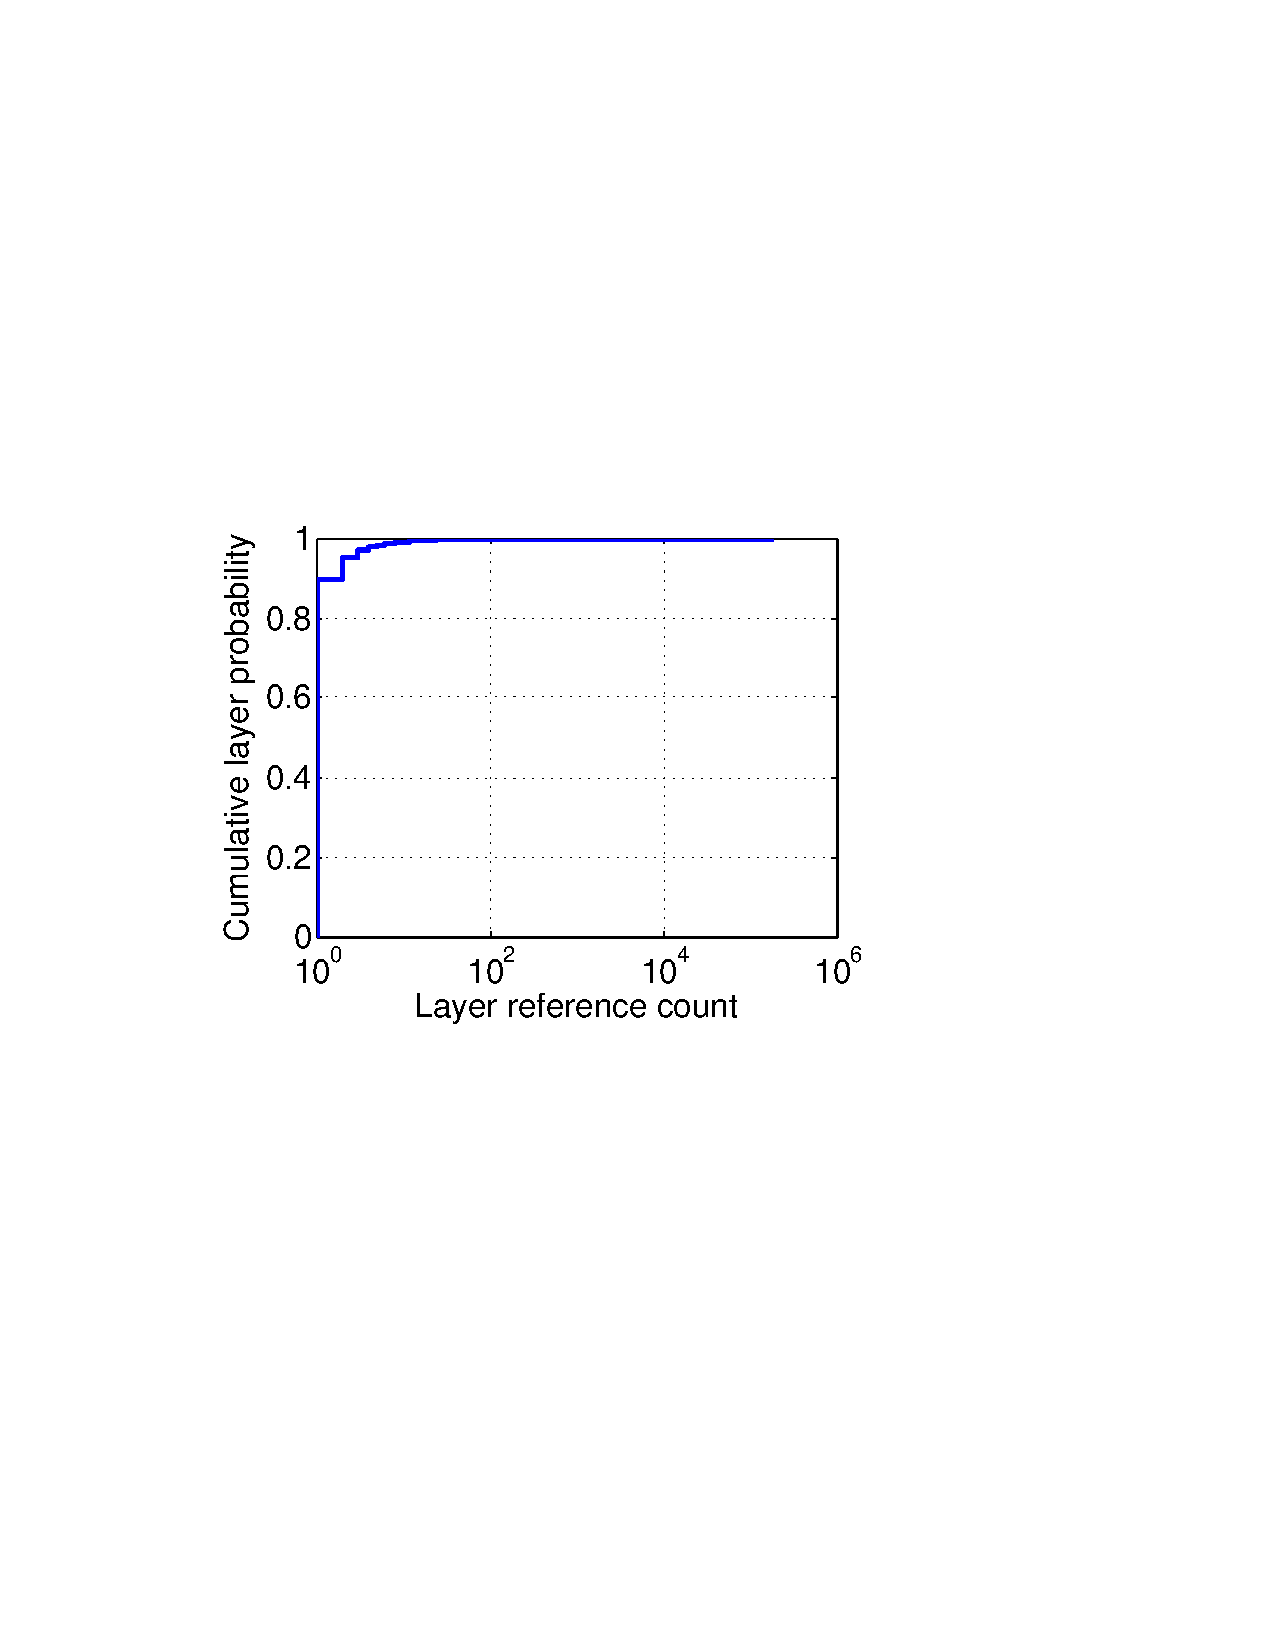
\includegraphics[width=1\textwidth]{graphs/shared-cnt-cdf.pdf}
			\caption{CDF of layer\\\ reference count.}
			\label{fig:ref_count}
		\end{minipage}
	\begin{minipage}{0.22\textwidth}
		\centering
		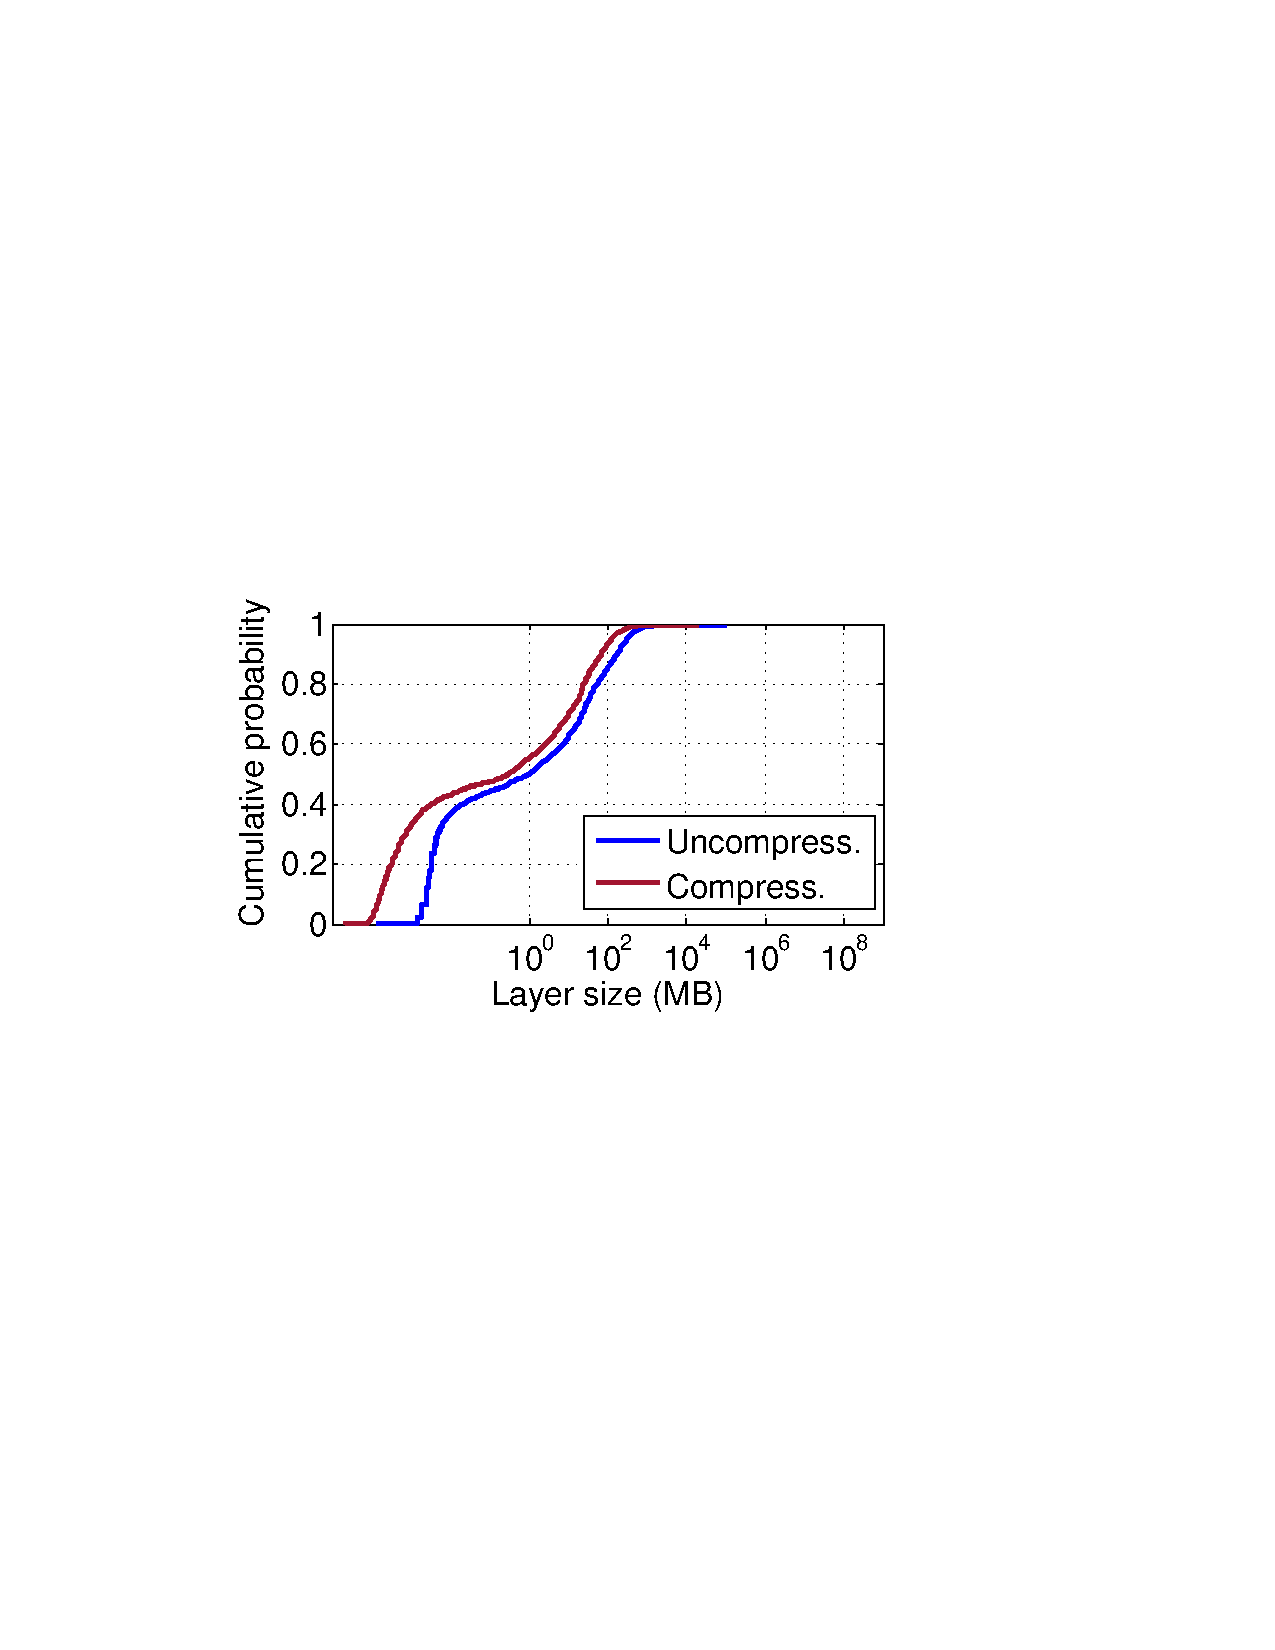
\includegraphics[width=1\textwidth]{graphs/layer-size-cdf.pdf}
		\caption{CDF of compress. and uncompress. layer size.}
		\label{fig:layer-size-cdf}
	\end{minipage}
\end{figure}

%
%+-----------------------------------------------------------------------+----------------+
%|layer_id                                                               |shared_image_cnt|
%+-----------------------------------------------------------------------+----------------+
%|sha256:a3ed95caeb02ffe68cdd9fd84406680ae93d633cb16422d00e8a7c22955b46d4|184171          | empty
%|sha256:e190868d63f8f8b85b026e53b5724c3c2a4548e1d642953442559cfa5f79b2c9|33413           | ubuntu 14.04.2 LTS. 
%|sha256:909cd34c6fd77d398af1d93e9d4f7f76104903f237be3d4db7b345a19631f291|33323           | dpkg
%|sha256:0b9bfabab7c119abe303f22a146ff78be4ab0abdc798b0a0e97e94e80238a7e8|33295           | apt
%|sha256:8eed3712d2cfd8c37b19d324452ba9cdb445933c04c9175c4e945b0d7241f1e3|31517           | cowsay
%|sha256:c57b6bcc83e3e88fb3748ea3f0cb13d77c4e2ffa7b9a8ded3d636f17d2d83759|31503           | cowsay 3.03 installasion package
%|sha256:8978f6879e2f86eb7a063e70f7d89feecde9950c40fc68f1f53d00b3c8ce9b52|31179           | same cowsay but different git info
%|sha256:00bf65475aba8f1077fa9629f088a5f531d645faeccb6acd7a8626c7d896a4c4|29200           | (looks like linux distribution)

\paragraph{Compression}
%
Figure~\ref{fig:layer-size-cdf} presents compressed and uncompressed layer size
distributions.
%
We found that 50\% of the layers are smaller than 1MB and 90\% of the layers are
smaller than 64MB in compressed format.
%
If uncompressed, 50\% of the layers are smaller than 2 MB and 90\% of the
layers are smaller than 170MB.
%
Moreover, the total compressed layer dataset grows from 47~TB to 167~TB after decompression, resulting in \textbf{3.6$\times$} compression ratio.

\paragraph{File-level deduplication}
%
Next, we calculate deduplication ratio in terms of file count and capacity for
the complete unpacked dataset.
%
After removing redundant files, there are only 3.2\% of files left that occupy
24~TB, resulting in deduplication ratios of \textbf{31.5$\times$} and
\textbf{6.9$\times$} in terms of file count and capacity, respectively.
%
%\begin{figure} \centering
%	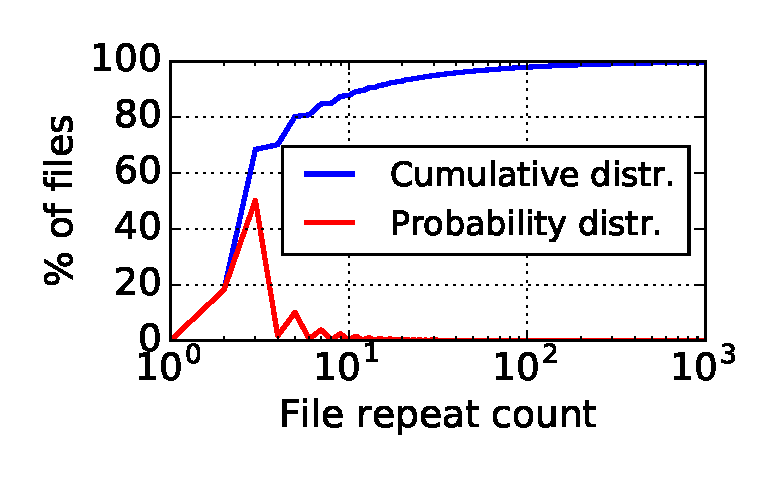
\includegraphics[width=0.45\textwidth]{graphs/File_repeat_count.eps}
%	\caption{File repeat count distribution.
%	%
%	\VT{No need for Y2}
%	%
%	\VT{Still need to use \% on the axis}\NZ{addressed both}
%	%
%	} \label{fig:file-repeat-cnt}
%\end{figure}

\begin{figure}[t]
	\centering
	\begin{minipage}{0.35\textwidth}
		\centering
		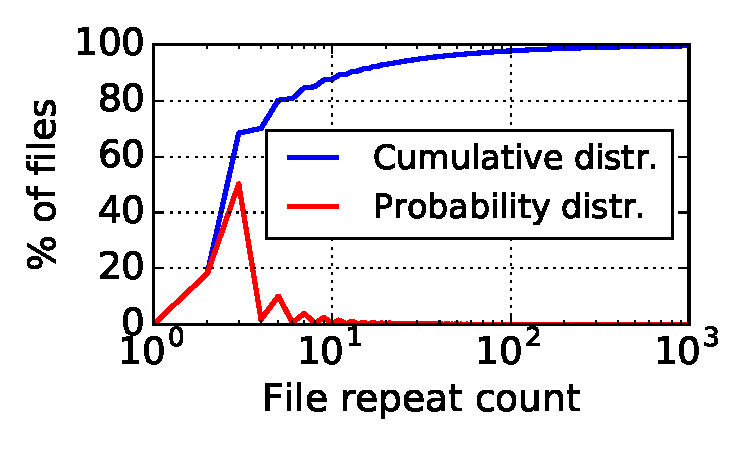
\includegraphics[width=1\textwidth]{graphs/File_repeat_count-eps.pdf}
		\caption{File repeat count distribution.
		}
		%\vspace{15pt}
		\label{fig:file-repeat-cnt}
	\end{minipage}
	\begin{minipage}{0.35\textwidth}
		\centering
		%\vspace{-10pt}
		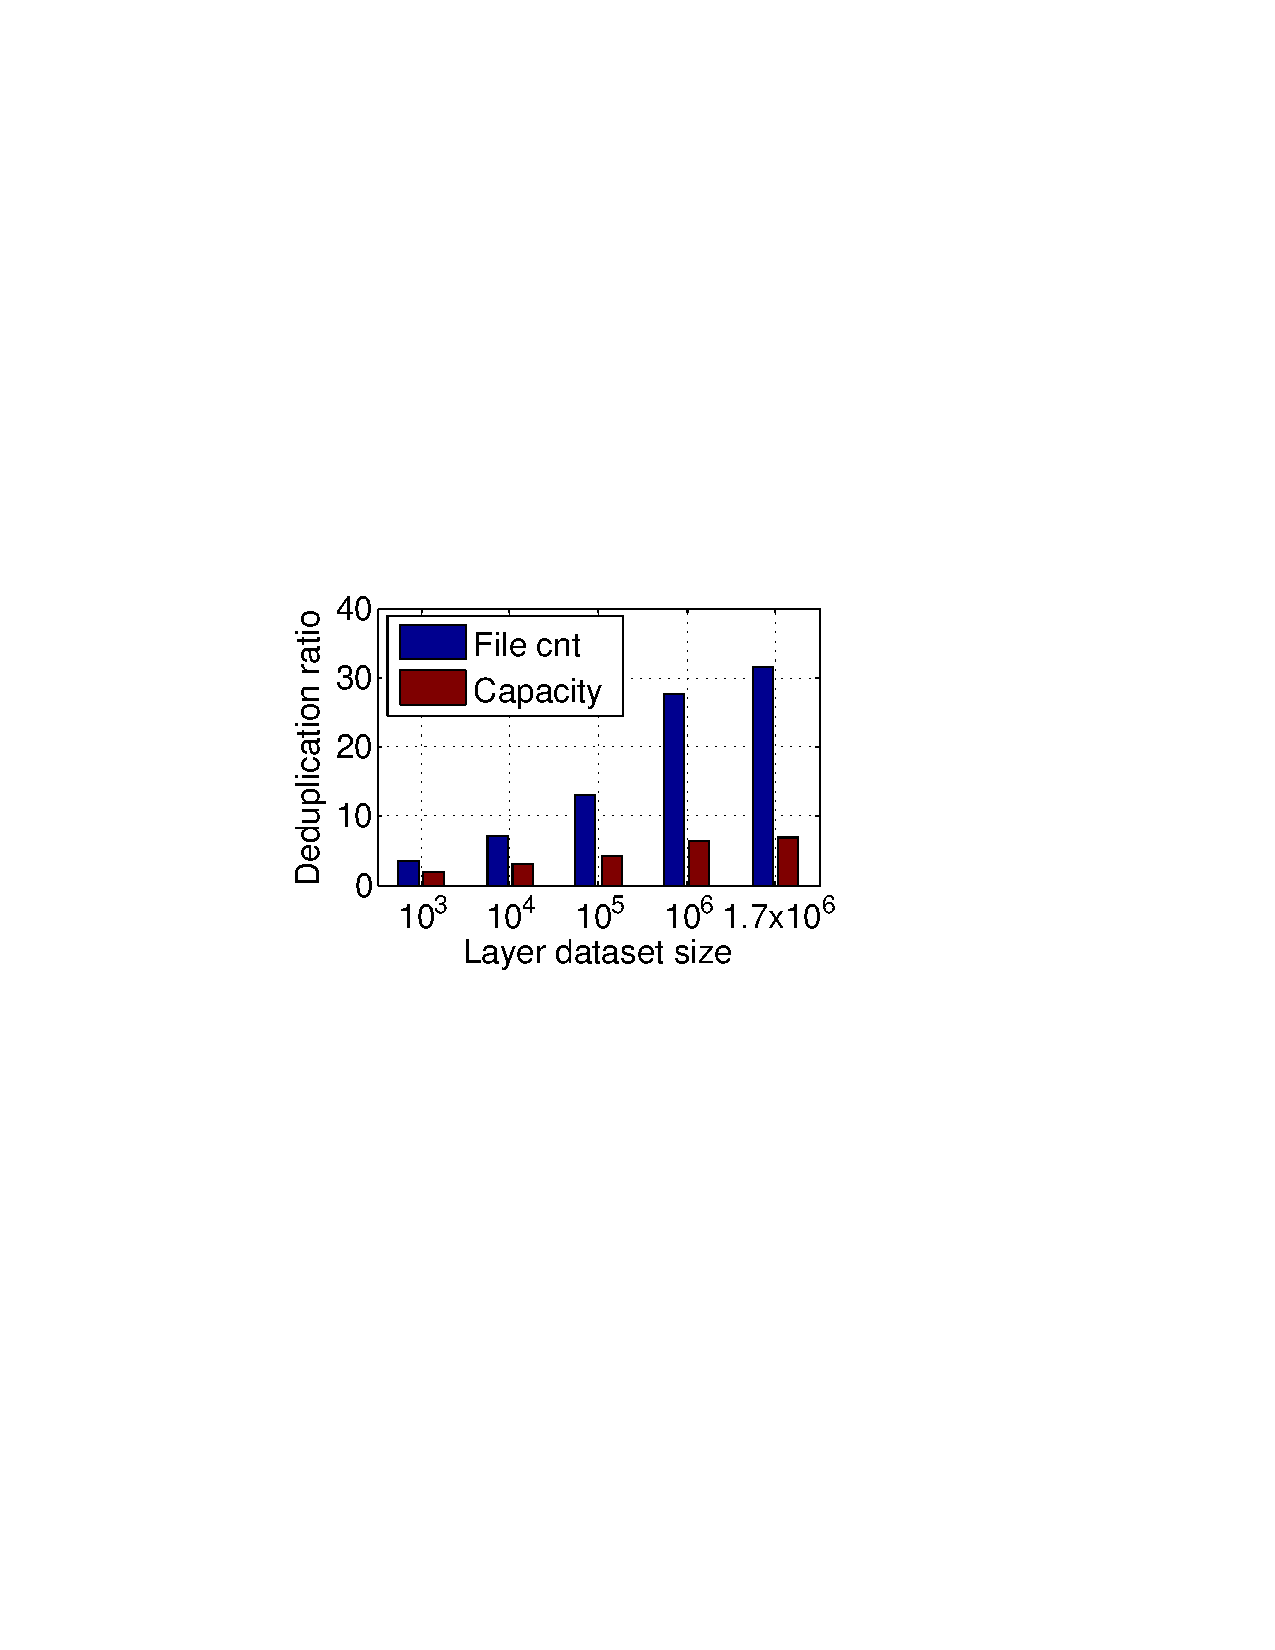
\includegraphics[width=1\textwidth]{graphs/dedup-ratio-grow} 
		\caption{Deduplication ratio growth.
		} 
		\vspace{-2pt}
		\label{fig:dedup-ratio-growth}
	\end{minipage}
\end{figure}

%\begin{figure} 
%	\centering
%	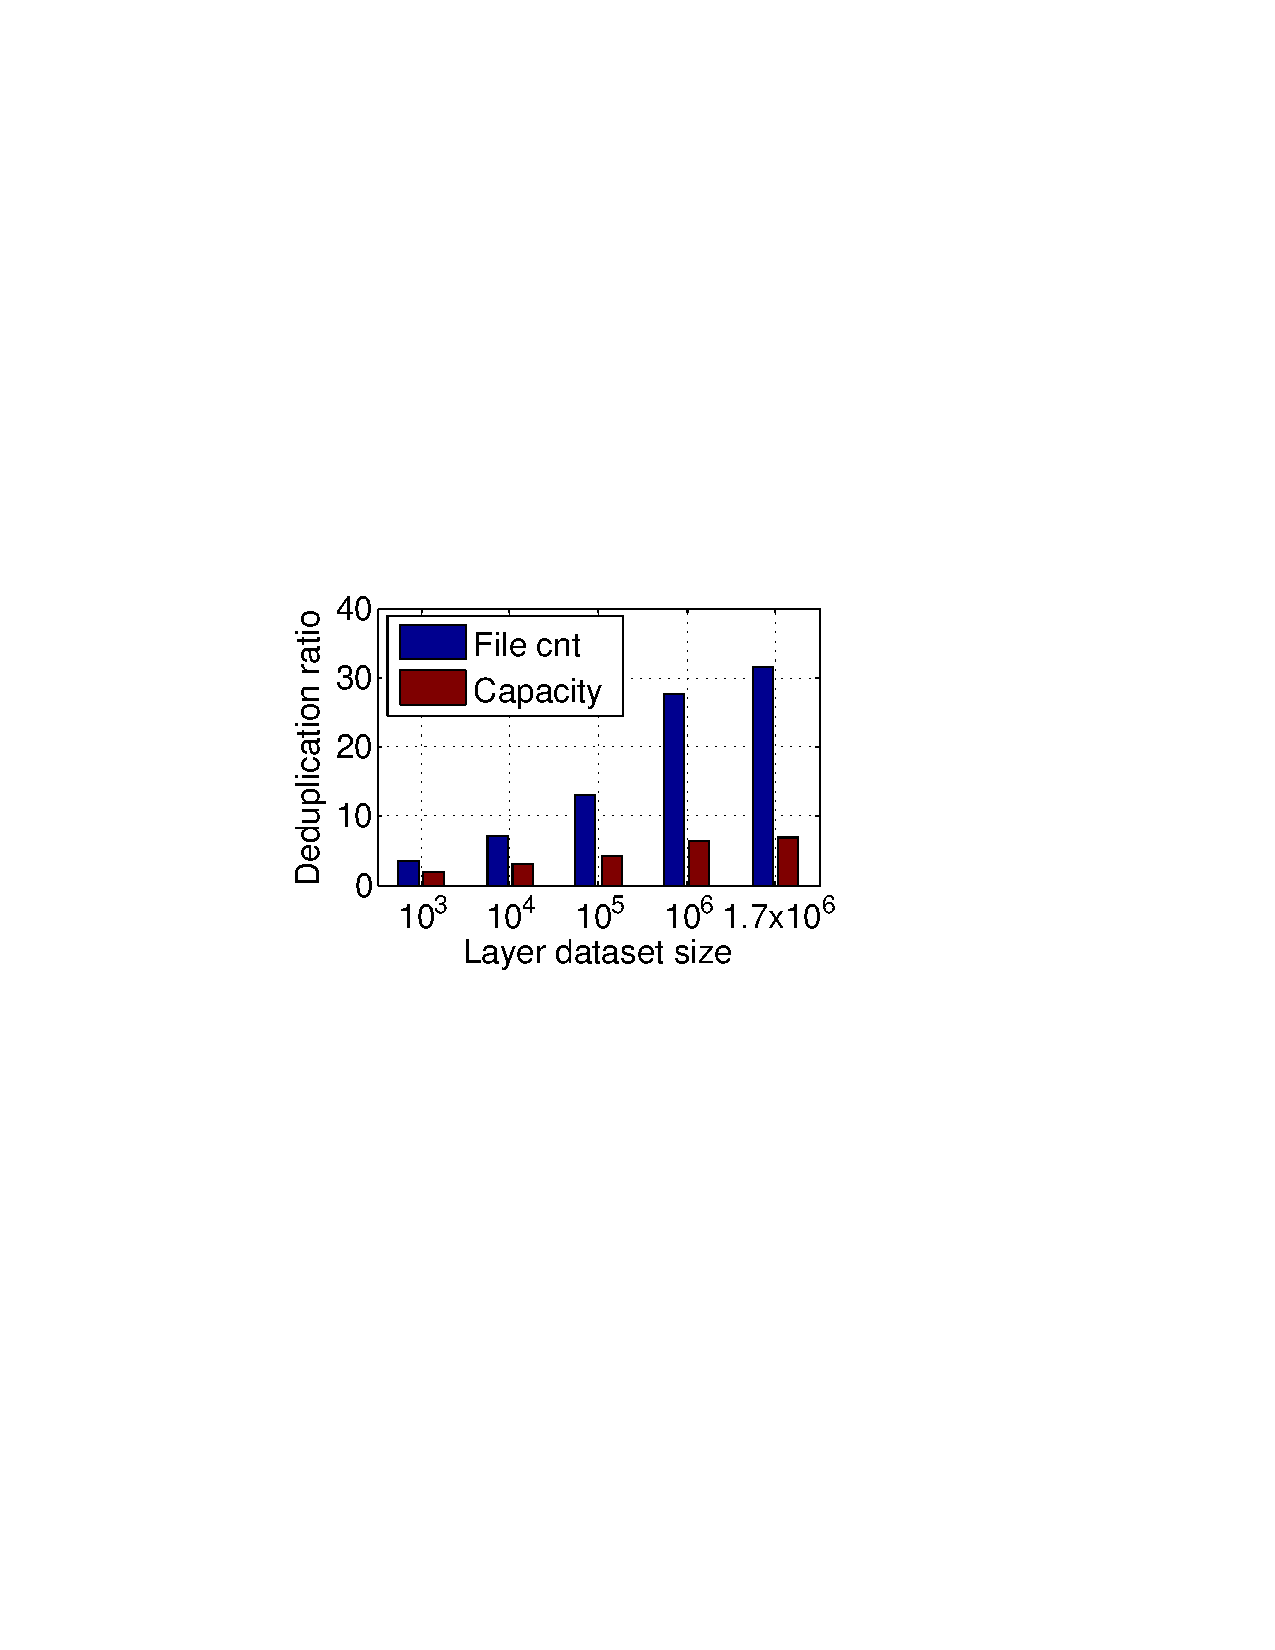
\includegraphics[width=0.25\textwidth]{graphs/dedup-ratio-grow} 
%	\caption{The growth of deduplication ratio.
%	} 
%	\label{fig:dedup-ratio-growth} 
%\end{figure}

%
We further analyzed the repeat count for every file.
%
Figure~\ref{fig:file-repeat-cnt} shows the distributions of file repeat count.  
%
We see that over 99.4\% of files have more than one copy.
%
Around 50\% of files have exactly 4 copies and 90\% of files have 10 or less
copies. 
%
The file that has the maximum repeat count 53,654,306---is an empty file.
%Other hot redundant files are 
%
%\VT{Do we know anything about those empty files}.\NZ{addressed}
Around 4\% of empty files are \texttt{\_\_init\_\_.py}, which make Python treat the 
directories as containing packages and are usually empty files. 
Other frequent empty files include empty \texttt{lock} files, \texttt{.gitkeep}, etc.

We also analyze 5 frequently repeated files which repeat 3,338,145 -- 11,847,356 times.
Specifically, two files 
\texttt{libkrb5-3:amd64.postrm} and \texttt{libkrb5-3:amd64.postinst}
are two MIT Kerberos runtime libraries for \texttt{dpkg}.
Another two files \texttt{license} and \texttt{.npmignore} are related to \texttt{npm} package manager.
The last file \texttt{dependency\_links.txt} contains a list of dependency URLs for Python.

\paragraph{Deduplication ratio growth with layer dataset size}

Figure~\ref{fig:dedup-ratio-growth} shows the deduplication ratio growth over the layer dataset size. The x-axis values correspond to the size of 4 random samples from our whole dataset. We see that deduplication ratio increases with the layer dataset size.
%
For example, deduplication ratio
in terms of file count increases from \textbf{3.6$\times$} to \textbf{31.5$\times$} while the deduplication ratio in terms of capacity increases from \textbf{1.9$\times$} to \textbf{6.9$\times$}  
as the layer dataset grows from 1000 to 1.7 million.
% 
As the number of images stored in the Docker registry increases dramatically,
file-level deduplication can provide significant storage space savings.
